% Important: If latex complains about unicode characters,
% please use "\usepackage[utf8x]{inputenc}" in your preamble
% You can change the size of the picture by putting it into the construct:
% 1) \resizebox{10cm}{!}{"below picture"} to scale horizontally to 10 cm
% 2) \resizebox{!}{15cm}{"below picture"} to scale vertically to 15 cm
% 3) \resizebox{10cm}{15cm}{"below picture"} a combination of above two
% It is not recomended to use the scale option of the tikzpicture environment.
\scalebox{0.35}{
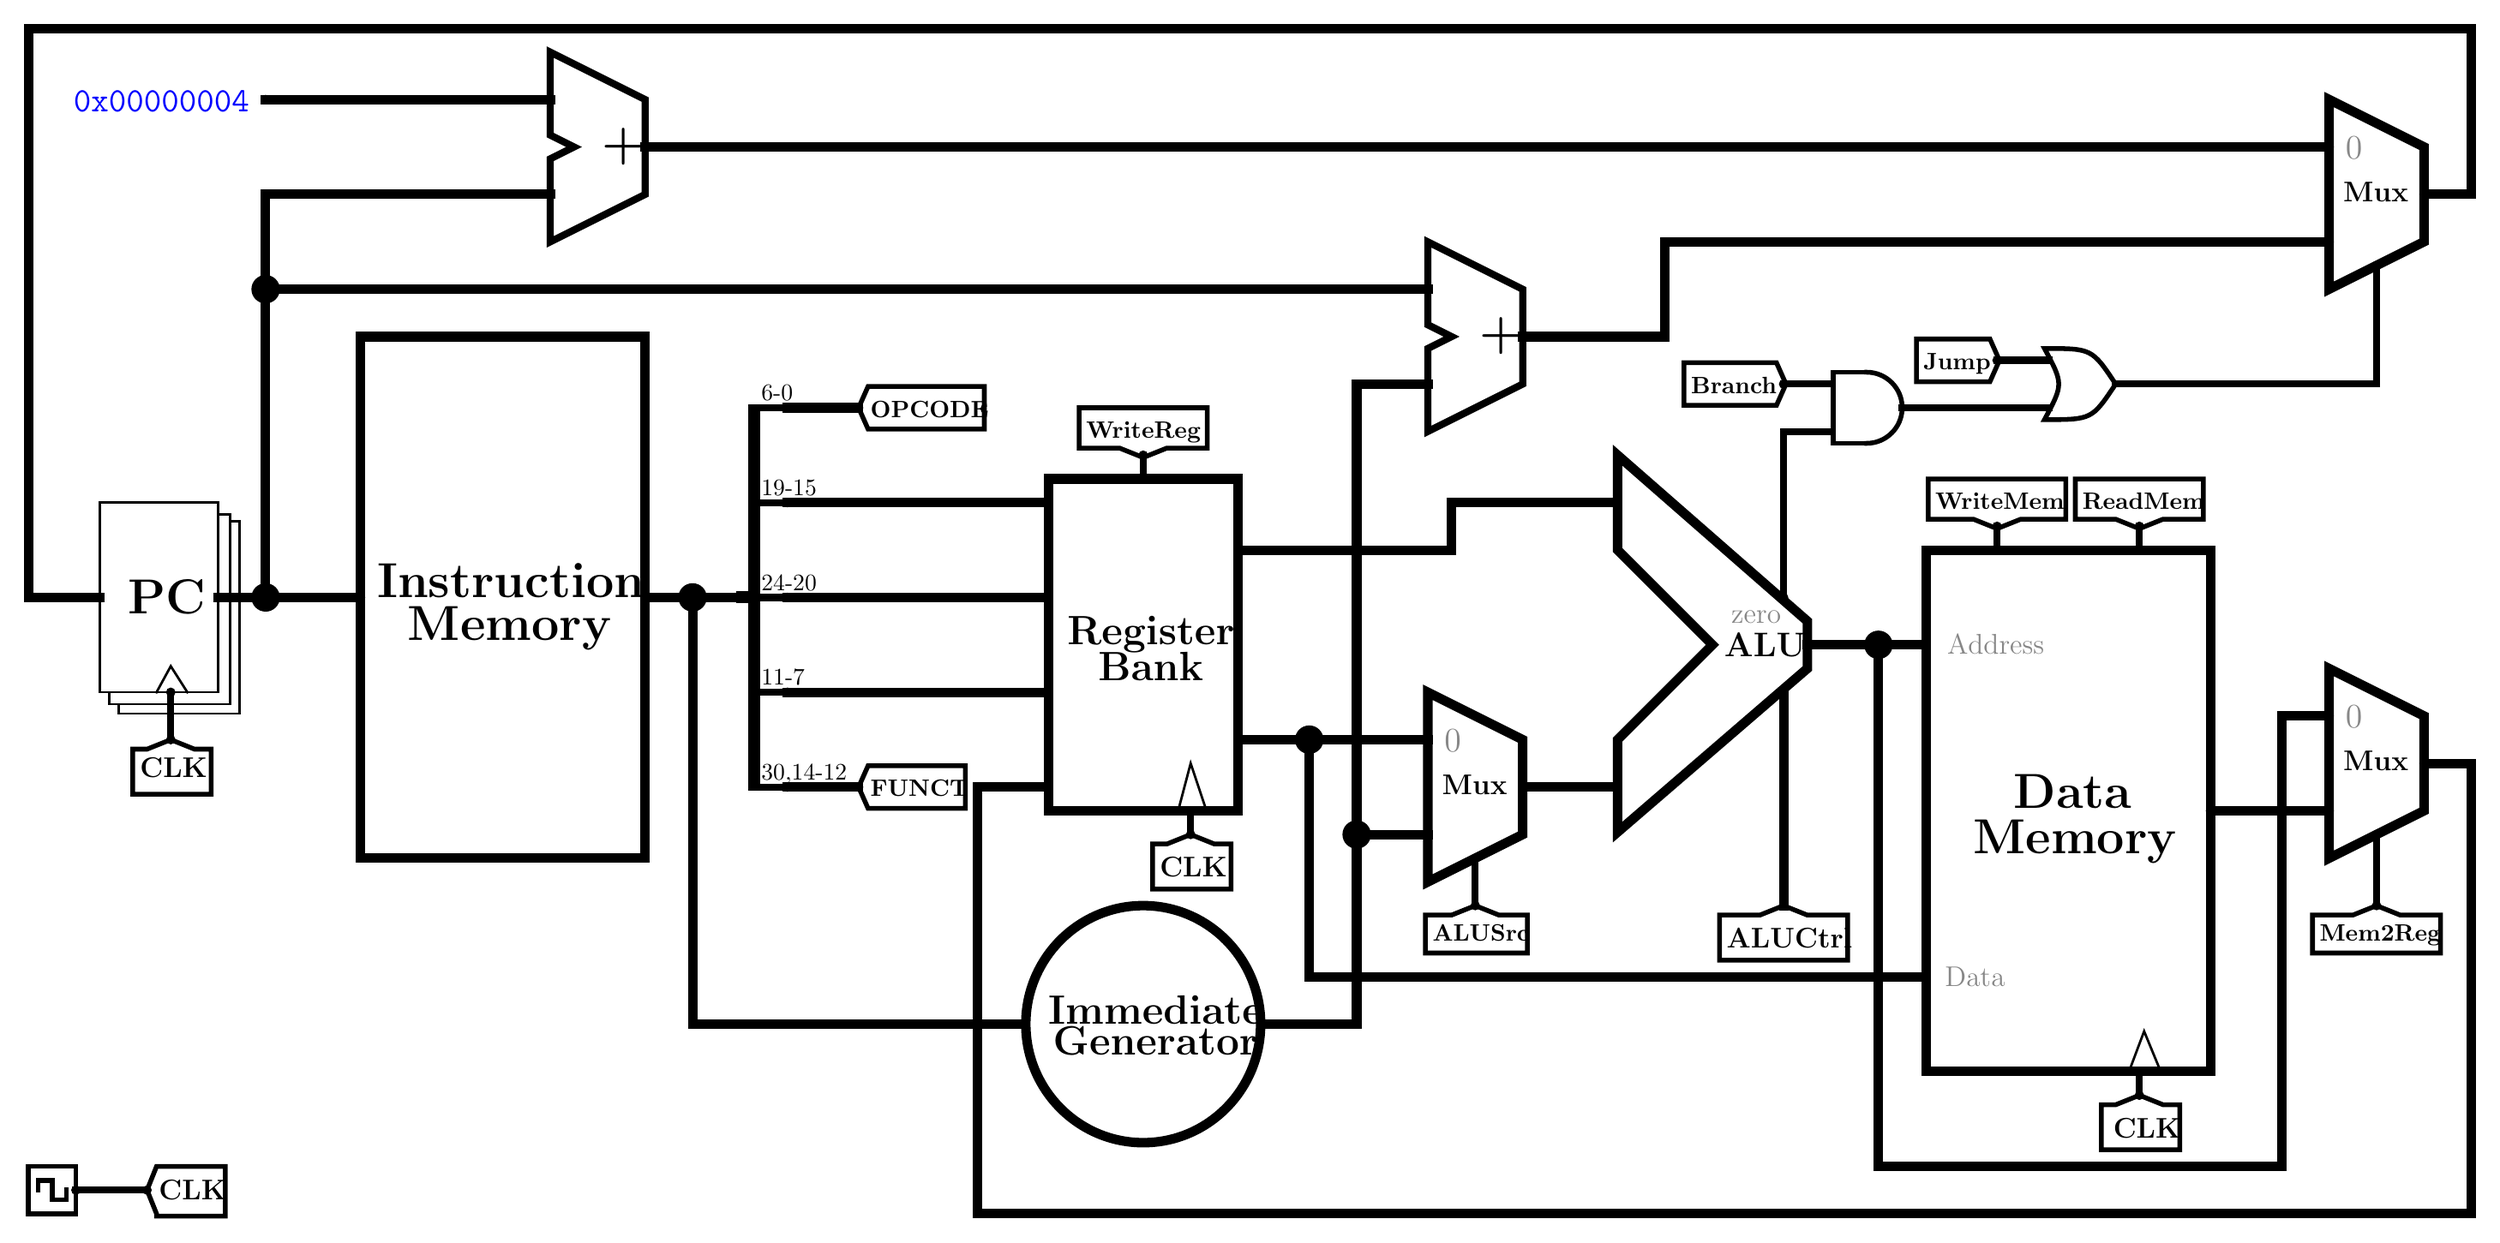
\begin{tikzpicture}[x=1pt,y=-1pt,line cap=rect]
\def\logisimfontA#1{{\fontspec{CMU Serif}#1}} % cmr equivalent
\def\logisimfontB#1{{\fontspec{CMU Bright}#1}}
\def\logisimfontC#1{{\fontspec{CMU Bright}#1}}
\def\logisimfontD#1{{\fontspec{CMU Typewriter Text}#1}} % cmtt equivalent
\definecolor{custcol_87_87_87}{RGB}{135, 135, 135}
\definecolor{custcol_0_0_0}{RGB}{0, 0, 0}
\definecolor{custcol_ff_ff_ff}{RGB}{255, 255, 255}
\draw [line width=4.0pt, custcol_0_0_0 ]  (925.0,335.0) -- (975.0,335.0) ;
\draw [line width=3.0pt, custcol_0_0_0 ]  (895.0,445.0) -- (895.0,455.0) ;
\draw [line width=4.0pt, custcol_0_0_0 ]  (105.0,35.0) -- (225.0,35.0) ;
\draw [line width=3.0pt, custcol_0_0_0 ]  (475.0,185.0) -- (475.0,195.0) ;
\draw [line width=3.0pt, custcol_0_0_0 ]  (995.0,345.0) -- (995.0,375.0) ;
\draw [line width=4.0pt, custcol_0_0_0 ]  (745.0,285.0) -- (745.0,375.0) ;
\draw [line width=4.0pt, custcol_0_0_0 ]  (325.0,285.0) -- (435.0,285.0) ;
\draw [line width=4.0pt, custcol_0_0_0 ]  (325.0,205.0) -- (435.0,205.0) ;
\draw [line width=4.0pt, custcol_0_0_0 ]  (325.0,245.0) -- (435.0,245.0) ;
\draw [line width=3.0pt, custcol_0_0_0 ]  (25.0,495.0) -- (55.0,495.0) ;
\draw [line width=4.0pt, custcol_0_0_0 ]  (265.0,245.0) -- (285.0,245.0) -- (305.0,245.0) ;
\draw [line width=4.0pt, custcol_0_0_0 ]  (225.0,75.0) -- (105.0,75.0) -- (105.0,115.0) -- (105.0,245.0) -- (145.0,245.0) ;
\draw [line width=4.0pt, custcol_0_0_0 ]  (85.0,245.0) -- (105.0,245.0) ;
\draw [line width=4.0pt, custcol_0_0_0 ]  (755.0,265.0) -- (785.0,265.0) ;
\draw [line width=4.0pt, custcol_0_0_0 ]  (515.0,305.0) -- (545.0,305.0) -- (545.0,405.0) -- (805.0,405.0) ;
\draw [line width=4.0pt, custcol_0_0_0 ]  (595.0,155.0) -- (565.0,155.0) -- (565.0,345.0) -- (565.0,425.0) -- (525.0,425.0) ;
\draw [line width=3.0pt, custcol_0_0_0 ]  (495.0,335.0) -- (495.0,345.0) ;
\draw [line width=3.0pt, custcol_0_0_0 ]  (895.0,215.0) -- (895.0,225.0) ;
\draw [line width=4.0pt, custcol_0_0_0 ]  (545.0,305.0) -- (595.0,305.0) ;
\draw [line width=3.0pt, custcol_0_0_0 ]  (835.0,215.0) -- (835.0,225.0) ;
\draw [line width=4.0pt, custcol_0_0_0 ]  (635.0,325.0) -- (675.0,325.0) ;
\draw [line width=4.0pt, custcol_0_0_0 ]  (105.0,115.0) -- (595.0,115.0) ;
\draw [line width=3.0pt, custcol_0_0_0 ]  (65.0,285.0) -- (65.0,305.0) ;
\draw [line width=3.0pt, custcol_0_0_0 ]  (885.0,155.0) -- (995.0,155.0) -- (995.0,105.0) ;
\draw [line width=3.0pt, custcol_0_0_0 ]  (615.0,355.0) -- (615.0,375.0) ;
\draw [line width=3.0pt, custcol_0_0_0 ]  (745.0,245.0) -- (745.0,175.0) -- (765.0,175.0) ;
\draw [line width=3.0pt, custcol_0_0_0 ]  (745.0,155.0) -- (765.0,155.0) ;
\draw [line width=4.0pt, custcol_0_0_0 ]  (975.0,95.0) -- (695.0,95.0) -- (695.0,135.0) -- (635.0,135.0) ;
\draw [line width=4.0pt, custcol_0_0_0 ]  (325.0,325.0) -- (355.0,325.0) ;
\draw [line width=4.0pt, custcol_0_0_0 ]  (325.0,165.0) -- (355.0,165.0) ;
\draw [line width=4.0pt, custcol_0_0_0 ]  (565.0,345.0) -- (595.0,345.0) ;
\draw [line width=4.0pt, custcol_0_0_0 ]  (515.0,225.0) -- (605.0,225.0) -- (605.0,205.0) -- (675.0,205.0) ;
\draw [line width=4.0pt, custcol_0_0_0 ]  (285.0,245.0) -- (285.0,425.0) -- (425.0,425.0) ;
\draw [line width=4.0pt, custcol_0_0_0 ]  (975.0,295.0) -- (955.0,295.0) -- (955.0,485.0) -- (785.0,485.0) -- (785.0,265.0) -- (805.0,265.0) ;
\draw [line width=4.0pt, custcol_0_0_0 ]  (435.0,325.0) -- (405.0,325.0) -- (405.0,505.0) -- (1035.0,505.0) -- (1035.0,315.0) -- (1015.0,315.0) ;
\draw [line width=4.0pt, custcol_0_0_0 ]  (35.0,245.0) -- (5.0,245.0) -- (5.0,5.0) -- (1035.0,5.0) -- (1035.0,75.0) -- (1015.0,75.0) ;
\draw [line width=4.0pt, custcol_0_0_0 ]  (265.0,55.0) -- (975.0,55.0) ;
\fill [line width=4.0pt, custcol_0_0_0]  (285.0,245.0) ellipse (6.0 and 6.0 );
\fill [line width=4.0pt, custcol_0_0_0]  (105.0,245.0) ellipse (6.0 and 6.0 );
\fill [line width=4.0pt, custcol_0_0_0]  (565.0,345.0) ellipse (6.0 and 6.0 );
\fill [line width=4.0pt, custcol_0_0_0]  (785.0,265.0) ellipse (6.0 and 6.0 );
\fill [line width=4.0pt, custcol_0_0_0]  (105.0,115.0) ellipse (6.0 and 6.0 );
\fill [line width=4.0pt, custcol_0_0_0]  (545.0,305.0) ellipse (6.0 and 6.0 );
\draw [line width=4.0pt, custcol_0_0_0 ]  (145.0,135.0) -- (264.0,135.0) ;
\draw [line width=4.0pt, custcol_0_0_0 ]  (265.0,135.0) -- (265.0,354.0) ;
\draw [line width=4.0pt, custcol_0_0_0 ]  (265.0,355.0) -- (146.0,355.0) ;
\draw [line width=4.0pt, custcol_0_0_0 ]  (145.0,355.0) -- (145.0,136.0) ;
\logisimfontB{\fontsize{20pt}{20pt}\bfseries\selectfont\node[inner sep=0, outer sep=0, custcol_0_0_0, anchor=base west] at  (152.0,245.0)  {Instruction};}
\logisimfontB{\fontsize{20pt}{20pt}\bfseries\selectfont\node[inner sep=0, outer sep=0, custcol_0_0_0, anchor=base west] at  (165.0,263.0)  {Memory};}
\fill [line width=1.0pt, custcol_0_0_0]  (145.0,245.0) ellipse (2.0 and 2.0 );
\fill [line width=1.0pt, custcol_0_0_0]  (265.0,245.0) ellipse (2.0 and 2.0 );
\draw [line width=3.0pt, custcol_0_0_0 ]  (325.0,165.0) -- (311.0,165.0) ;
\draw [line width=3.0pt, custcol_0_0_0 ]  (325.0,205.0) -- (311.0,205.0) ;
\draw [line width=3.0pt, custcol_0_0_0 ]  (325.0,245.0) -- (311.0,245.0) ;
\draw [line width=3.0pt, custcol_0_0_0 ]  (325.0,285.0) -- (311.0,285.0) ;
\draw [line width=3.0pt, custcol_0_0_0 ]  (325.0,325.0) -- (311.0,325.0) ;
\draw [line width=5.0pt, custcol_0_0_0 ]  (306.0,245.0) -- (311.0,245.0) ;
\draw [line width=5.0pt, custcol_0_0_0 ]  (311.0,166.0) -- (311.0,324.0) ;
\logisimfontA{\fontsize{10pt}{10pt}\selectfont\node[inner sep=0, outer sep=0, custcol_0_0_0, anchor=base west] at  (314.0,162.0)  {6-0};}
\logisimfontA{\fontsize{10pt}{10pt}\selectfont\node[inner sep=0, outer sep=0, custcol_0_0_0, anchor=base west] at  (314.0,202.0)  {19-15};}
\logisimfontA{\fontsize{10pt}{10pt}\selectfont\node[inner sep=0, outer sep=0, custcol_0_0_0, anchor=base west] at  (314.0,242.0)  {24-20};}
\logisimfontA{\fontsize{10pt}{10pt}\selectfont\node[inner sep=0, outer sep=0, custcol_0_0_0, anchor=base west] at  (314.0,282.0)  {11-7};}
\logisimfontA{\fontsize{10pt}{10pt}\selectfont\node[inner sep=0, outer sep=0, custcol_0_0_0, anchor=base west] at  (314.0,322.0)  {30,14-12};}
\fill [line width=5.0pt, custcol_0_0_0]  (305.0,245.0) ellipse (2.0 and 2.0 );
\fill [line width=5.0pt, custcol_0_0_0]  (325.0,165.0) ellipse (2.0 and 2.0 );
\fill [line width=5.0pt, custcol_0_0_0]  (325.0,205.0) ellipse (2.0 and 2.0 );
\fill [line width=5.0pt, custcol_0_0_0]  (325.0,245.0) ellipse (2.0 and 2.0 );
\fill [line width=5.0pt, custcol_0_0_0]  (325.0,285.0) ellipse (2.0 and 2.0 );
\fill [line width=5.0pt, custcol_0_0_0]  (325.0,325.0) ellipse (2.0 and 2.0 );
\draw [line width=4.0pt, custcol_0_0_0 ]  (595.0,285.0) -- (595.0,365.0) -- (635.0,345.0) -- (635.0,305.0) -- cycle;
\logisimfontC{\fontsize{14pt}{14pt}\selectfont\node[inner sep=0, outer sep=0, custcol_87_87_87, anchor=base west] at  (602.0,310.0)  {0};}
\logisimfontB{\fontsize{12pt}{12pt}\bfseries\selectfont\node[inner sep=0, outer sep=0, custcol_0_0_0, anchor=base west] at  (601.0,328.0)  {Mux};}
\fill [line width=1.0pt, custcol_0_0_0]  (595.0,305.0) ellipse (2.0 and 2.0 );
\fill [line width=1.0pt, custcol_0_0_0]  (595.0,345.0) ellipse (2.0 and 2.0 );
\fill [line width=1.0pt, custcol_0_0_0]  (615.0,355.0) ellipse (2.0 and 2.0 );
\fill [line width=1.0pt, custcol_0_0_0]  (635.0,325.0) ellipse (2.0 and 2.0 );
\logisimfontB{\fontsize{10pt}{10pt}\bfseries\selectfont\node[inner sep=0, outer sep=0, custcol_0_0_0, anchor=base west] at  (597.0,390.0)  {ALUSrc};}
\draw [line width=2.0pt, custcol_0_0_0 ]  (594.0,379.0) -- (605.0,379.0) -- (615.0,375.0) -- (625.0,379.0) -- (637.0,379.0) -- (637.0,395.0) -- (594.0,395.0) -- cycle;
\fill [line width=2.0pt, custcol_0_0_0]  (615.0,375.0) ellipse (2.0 and 2.0 );
\draw [line width=4.0pt, custcol_0_0_0 ]  (975.0,275.0) -- (975.0,355.0) -- (1015.0,335.0) -- (1015.0,295.0) -- cycle;
\logisimfontC{\fontsize{14pt}{14pt}\selectfont\node[inner sep=0, outer sep=0, custcol_87_87_87, anchor=base west] at  (982.0,300.0)  {0};}
\logisimfontB{\fontsize{12pt}{12pt}\bfseries\selectfont\node[inner sep=0, outer sep=0, custcol_0_0_0, anchor=base west] at  (981.0,318.0)  {Mux};}
\fill [line width=1.0pt, custcol_0_0_0]  (975.0,295.0) ellipse (2.0 and 2.0 );
\fill [line width=1.0pt, custcol_0_0_0]  (975.0,335.0) ellipse (2.0 and 2.0 );
\fill [line width=1.0pt, custcol_0_0_0]  (995.0,345.0) ellipse (2.0 and 2.0 );
\fill [line width=1.0pt, custcol_0_0_0]  (1015.0,315.0) ellipse (2.0 and 2.0 );
\logisimfontB{\fontsize{10pt}{10pt}\bfseries\selectfont\node[inner sep=0, outer sep=0, custcol_0_0_0, anchor=base west] at  (971.0,390.0)  {Mem2Reg};}
\draw [line width=2.0pt, custcol_0_0_0 ]  (968.0,379.0) -- (985.0,379.0) -- (995.0,375.0) -- (1005.0,379.0) -- (1022.0,379.0) -- (1022.0,395.0) -- (968.0,395.0) -- cycle;
\fill [line width=2.0pt, custcol_0_0_0]  (995.0,375.0) ellipse (2.0 and 2.0 );
\draw [line width=3.0pt, custcol_0_0_0 ]  (225.0,15.0) -- (225.0,50.0) -- (235.0,55.0) -- (225.0,60.0) -- (225.0,95.0) -- (265.0,75.0) -- (265.0,35.0) -- cycle;
\logisimfontB{\fontsize{20pt}{20pt}\bfseries\selectfont\node[inner sep=0, outer sep=0, custcol_0_0_0, anchor=base west] at  (247.0,60.0)  {+};}
\fill [line width=1.0pt, custcol_0_0_0]  (225.0,35.0) ellipse (2.0 and 2.0 );
\fill [line width=1.0pt, custcol_0_0_0]  (225.0,75.0) ellipse (2.0 and 2.0 );
\fill [line width=1.0pt, custcol_0_0_0]  (265.0,55.0) ellipse (2.0 and 2.0 );
\logisimfontD{\fontsize{14pt}{14pt}\selectfont\node[inner sep=0, outer sep=0, custcol_0_0_0, anchor=base west] at  (24.0,40.0)  {\textcolor{blue}{\texttt{0x00000004}}};}
\fill [line width=1.0pt, custcol_0_0_0]  (105.0,35.0) ellipse (2.0 and 2.0 );
\logisimfontB{\fontsize{10pt}{10pt}\bfseries\selectfont\node[inner sep=0, outer sep=0, custcol_0_0_0, anchor=base west] at  (809.0,208.0)  {WriteMem};}
\draw [line width=2.0pt, custcol_0_0_0 ]  (806.0,195.0) -- (864.0,195.0) -- (864.0,212.0) -- (845.0,212.0) -- (835.0,216.0) -- (825.0,212.0) -- (806.0,212.0) -- cycle;
\fill [line width=2.0pt, custcol_0_0_0]  (835.0,215.0) ellipse (2.0 and 2.0 );
\draw [line width=4.0pt, custcol_0_0_0 ]  (435.0,195.0) -- (514.0,195.0) ;
\draw [line width=4.0pt, custcol_0_0_0 ]  (515.0,195.0) -- (515.0,334.0) ;
\draw [line width=4.0pt, custcol_0_0_0 ]  (515.0,335.0) -- (436.0,335.0) ;
\draw [line width=4.0pt, custcol_0_0_0 ]  (435.0,335.0) -- (435.0,196.0) ;
\logisimfontB{\fontsize{16pt}{16pt}\bfseries\selectfont\node[inner sep=0, outer sep=0, custcol_0_0_0, anchor=base west] at  (443.0,265.0)  {Register};}
\logisimfontB{\fontsize{16pt}{16pt}\bfseries\selectfont\node[inner sep=0, outer sep=0, custcol_0_0_0, anchor=base west] at  (456.0,280.0)  {Bank};}
\draw [line width=1.0pt, custcol_0_0_0 ]  (490.0,334.0) -- (495.0,315.0) -- (501.0,333.0) ;
\fill [line width=1.0pt, custcol_0_0_0]  (435.0,205.0) ellipse (2.0 and 2.0 );
\fill [line width=1.0pt, custcol_0_0_0]  (435.0,245.0) ellipse (2.0 and 2.0 );
\fill [line width=1.0pt, custcol_0_0_0]  (435.0,285.0) ellipse (2.0 and 2.0 );
\fill [line width=1.0pt, custcol_0_0_0]  (435.0,325.0) ellipse (2.0 and 2.0 );
\fill [line width=1.0pt, custcol_0_0_0]  (475.0,195.0) ellipse (2.0 and 2.0 );
\fill [line width=1.0pt, custcol_0_0_0]  (495.0,335.0) ellipse (2.0 and 2.0 );
\fill [line width=1.0pt, custcol_0_0_0]  (515.0,225.0) ellipse (2.0 and 2.0 );
\fill [line width=1.0pt, custcol_0_0_0]  (515.0,305.0) ellipse (2.0 and 2.0 );
\logisimfontB{\fontsize{10pt}{10pt}\bfseries\selectfont\node[inner sep=0, outer sep=0, custcol_0_0_0, anchor=base west] at  (360.0,329.0)  {FUNCT};}
\draw [line width=2.0pt, custcol_0_0_0 ]  (359.0,316.0) -- (400.0,316.0) -- (400.0,334.0) -- (359.0,334.0) -- (355.0,325.0) -- cycle;
\fill [line width=2.0pt, custcol_0_0_0]  (355.0,325.0) ellipse (2.0 and 2.0 );
\logisimfontB{\fontsize{10pt}{10pt}\bfseries\selectfont\node[inner sep=0, outer sep=0, custcol_0_0_0, anchor=base west] at  (360.0,169.0)  {OPCODE};}
\draw [line width=2.0pt, custcol_0_0_0 ]  (359.0,156.0) -- (408.0,156.0) -- (408.0,174.0) -- (359.0,174.0) -- (355.0,165.0) -- cycle;
\fill [line width=2.0pt, custcol_0_0_0]  (355.0,165.0) ellipse (2.0 and 2.0 );
\logisimfontB{\fontsize{10pt}{10pt}\bfseries\selectfont\node[inner sep=0, outer sep=0, custcol_0_0_0, anchor=base west] at  (451.0,178.0)  {WriteReg};}
\draw [line width=2.0pt, custcol_0_0_0 ]  (448.0,165.0) -- (502.0,165.0) -- (502.0,182.0) -- (485.0,182.0) -- (475.0,186.0) -- (465.0,182.0) -- (448.0,182.0) -- cycle;
\fill [line width=2.0pt, custcol_0_0_0]  (475.0,185.0) ellipse (2.0 and 2.0 );
\logisimfontB{\fontsize{12pt}{12pt}\bfseries\selectfont\node[inner sep=0, outer sep=0, custcol_0_0_0, anchor=base west] at  (482.0,363.0)  {CLK};}
\draw [line width=2.0pt, custcol_0_0_0 ]  (479.0,349.0) -- (485.0,349.0) -- (495.0,345.0) -- (505.0,349.0) -- (512.0,349.0) -- (512.0,368.0) -- (479.0,368.0) -- cycle;
\fill [line width=2.0pt, custcol_0_0_0]  (495.0,345.0) ellipse (2.0 and 2.0 );
\logisimfontB{\fontsize{12pt}{12pt}\bfseries\selectfont\node[inner sep=0, outer sep=0, custcol_0_0_0, anchor=base west] at  (884.0,473.0)  {CLK};}
\draw [line width=2.0pt, custcol_0_0_0 ]  (879.0,459.0) -- (885.0,459.0) -- (895.0,455.0) -- (905.0,459.0) -- (912.0,459.0) -- (912.0,478.0) -- (879.0,478.0) -- cycle;
\fill [line width=2.0pt, custcol_0_0_0]  (895.0,455.0) ellipse (2.0 and 2.0 );
\draw [line width=1.0pt, custcol_0_0_0 ]  (35.0,205.0) -- (84.0,205.0) ;
\draw [line width=1.0pt, custcol_0_0_0 ]  (85.0,205.0) -- (85.0,284.0) ;
\draw [line width=1.0pt, custcol_0_0_0 ]  (85.0,285.0) -- (36.0,285.0) ;
\draw [line width=1.0pt, custcol_0_0_0 ]  (35.0,285.0) -- (35.0,206.0) ;
\draw [line width=1.0pt, custcol_0_0_0 ]  (59.0,285.0) -- (65.0,274.0) -- (72.0,285.0) ;
\logisimfontB{\fontsize{20pt}{20pt}\bfseries\selectfont\node[inner sep=0, outer sep=0, custcol_0_0_0, anchor=base west] at  (47.0,252.0)  {PC};}
\draw [line width=1.0pt, custcol_0_0_0 ]  (85.0,210.0) -- (90.0,210.0) -- (90.0,290.0) -- (39.0,290.0) -- (39.0,285.0) ;
\draw [line width=1.0pt, custcol_0_0_0 ]  (91.0,213.0) -- (94.0,213.0) -- (94.0,294.0) -- (43.0,294.0) -- (43.0,291.0) ;
\fill [line width=1.0pt, custcol_0_0_0]  (35.0,245.0) ellipse (2.0 and 2.0 );
\fill [line width=1.0pt, custcol_0_0_0]  (65.0,285.0) ellipse (2.0 and 2.0 );
\fill [line width=1.0pt, custcol_0_0_0]  (85.0,245.0) ellipse (2.0 and 2.0 );
\logisimfontB{\fontsize{12pt}{12pt}\bfseries\selectfont\node[inner sep=0, outer sep=0, custcol_0_0_0, anchor=base west] at  (52.0,321.0)  {CLK};}
\draw [line width=2.0pt, custcol_0_0_0 ]  (49.0,309.0) -- (55.0,309.0) -- (65.0,305.0) -- (75.0,309.0) -- (82.0,309.0) -- (82.0,328.0) -- (49.0,328.0) -- cycle;
\fill [line width=2.0pt, custcol_0_0_0]  (65.0,305.0) ellipse (2.0 and 2.0 );
\logisimfontB{\fontsize{12pt}{12pt}\bfseries\selectfont\node[inner sep=0, outer sep=0, custcol_0_0_0, anchor=base west] at  (60.0,499.0)  {CLK};}
\draw [line width=2.0pt, custcol_0_0_0 ]  (59.0,485.0) -- (88.0,485.0) -- (88.0,506.0) -- (59.0,506.0) -- (59.0,505.0) -- (55.0,495.0) -- cycle;
\fill [line width=2.0pt, custcol_0_0_0]  (55.0,495.0) ellipse (2.0 and 2.0 );
\draw [line width=2.0pt, custcol_0_0_0 ]  (5.0,485.0) -- (24.0,485.0) ;
\draw [line width=2.0pt, custcol_0_0_0 ]  (25.0,485.0) -- (25.0,504.0) ;
\draw [line width=2.0pt, custcol_0_0_0 ]  (25.0,505.0) -- (6.0,505.0) ;
\draw [line width=2.0pt, custcol_0_0_0 ]  (5.0,505.0) -- (5.0,486.0) ;
\draw [line width=2.0pt, custcol_0_0_0 ]  (9.0,495.0) -- (9.0,491.0) -- (15.0,491.0) -- (15.0,499.0) -- (21.0,499.0) -- (21.0,495.0) ;
\fill [line width=2.0pt, custcol_0_0_0]  (25.0,495.0) ellipse (2.0 and 2.0 );
\draw [line width=4.0pt, custcol_0_0_0]  (475.0,425.0) ellipse (49.5 and 50.0 );
\logisimfontB{\fontsize{16pt}{16pt}\bfseries\selectfont\node[inner sep=0, outer sep=0, custcol_0_0_0, anchor=base west] at  (435.0,425.0)  {Immediate};}
\logisimfontB{\fontsize{16pt}{16pt}\bfseries\selectfont\node[inner sep=0, outer sep=0, custcol_0_0_0, anchor=base west] at  (437.0,438.0)  {Generator};}
\fill [line width=1.0pt, custcol_0_0_0]  (425.0,425.0) ellipse (2.0 and 2.0 );
\fill [line width=1.0pt, custcol_0_0_0]  (525.0,425.0) ellipse (2.0 and 2.0 );
\logisimfontB{\fontsize{12pt}{12pt}\bfseries\selectfont\node[inner sep=0, outer sep=0, custcol_0_0_0, anchor=base west] at  (721.0,393.0)  {ALUCtrl};}
\draw [line width=2.0pt, custcol_0_0_0 ]  (718.0,379.0) -- (735.0,379.0) -- (745.0,375.0) -- (755.0,379.0) -- (772.0,379.0) -- (772.0,398.0) -- (718.0,398.0) -- cycle;
\fill [line width=2.0pt, custcol_0_0_0]  (745.0,375.0) ellipse (2.0 and 2.0 );
\draw [line width=4.0pt, custcol_0_0_0 ]  (975.0,35.0) -- (975.0,115.0) -- (1015.0,95.0) -- (1015.0,55.0) -- cycle;
\logisimfontC{\fontsize{14pt}{14pt}\selectfont\node[inner sep=0, outer sep=0, custcol_87_87_87, anchor=base west] at  (982.0,60.0)  {0};}
\logisimfontB{\fontsize{12pt}{12pt}\bfseries\selectfont\node[inner sep=0, outer sep=0, custcol_0_0_0, anchor=base west] at  (981.0,78.0)  {Mux};}
\fill [line width=1.0pt, custcol_0_0_0]  (975.0,55.0) ellipse (2.0 and 2.0 );
\fill [line width=1.0pt, custcol_0_0_0]  (975.0,95.0) ellipse (2.0 and 2.0 );
\fill [line width=1.0pt, custcol_0_0_0]  (995.0,105.0) ellipse (2.0 and 2.0 );
\fill [line width=1.0pt, custcol_0_0_0]  (1015.0,75.0) ellipse (2.0 and 2.0 );
\draw [line width=3.0pt, custcol_0_0_0 ]  (595.0,95.0) -- (595.0,130.0) -- (605.0,135.0) -- (595.0,140.0) -- (595.0,175.0) -- (635.0,155.0) -- (635.0,115.0) -- cycle;
\logisimfontB{\fontsize{20pt}{20pt}\bfseries\selectfont\node[inner sep=0, outer sep=0, custcol_0_0_0, anchor=base west] at  (617.0,140.0)  {+};}
\fill [line width=1.0pt, custcol_0_0_0]  (595.0,115.0) ellipse (2.0 and 2.0 );
\fill [line width=1.0pt, custcol_0_0_0]  (595.0,155.0) ellipse (2.0 and 2.0 );
\fill [line width=1.0pt, custcol_0_0_0]  (635.0,135.0) ellipse (2.0 and 2.0 );
\logisimfontB{\fontsize{10pt}{10pt}\bfseries\selectfont\node[inner sep=0, outer sep=0, custcol_0_0_0, anchor=base west] at  (871.0,208.0)  {ReadMem};}
\draw [line width=2.0pt, custcol_0_0_0 ]  (868.0,195.0) -- (922.0,195.0) -- (922.0,212.0) -- (905.0,212.0) -- (895.0,216.0) -- (885.0,212.0) -- (868.0,212.0) -- cycle;
\fill [line width=2.0pt, custcol_0_0_0]  (895.0,215.0) ellipse (2.0 and 2.0 );
\draw [line width=2.0pt, custcol_0_0_0] (780.0,180.0) arc (90.0:-90.0:15.0 and 15.0 );
\draw [line width=2.0pt, custcol_0_0_0 ]  (780.0,150.0) -- (766.0,150.0) -- (766.0,180.0) -- (780.0,180.0) ;
\logisimfontB{\fontsize{10pt}{10pt}\bfseries\selectfont\node[inner sep=0, outer sep=0, custcol_0_0_0, anchor=base west] at  (804.0,149.0)  {Jump};}
\draw [line width=2.0pt, custcol_0_0_0 ]  (801.0,136.0) -- (832.0,136.0) -- (836.0,145.0) -- (832.0,154.0) -- (801.0,154.0) -- cycle;
\fill [line width=2.0pt, custcol_0_0_0]  (835.0,145.0) ellipse (2.0 and 2.0 );
\draw [line width=3.0pt, custcol_0_0_0 ]  (835.0,145.0) -- (855.0,145.0) -- (857.0,145.0) ;
\draw [line width=3.0pt, custcol_0_0_0 ]  (795.0,165.0) -- (855.0,165.0) -- (857.0,165.0) ;
\draw [line width=2.0pt, custcol_0_0_0 ]  (885.0,155.0) .. controls  (875.0,140.0)  ..  (855.0,140.0) .. controls  (863.0,155.0)  ..  (855.0,170.0) .. controls  (875.0,170.0)  ..  (885.0,155.0) -- cycle ;
\logisimfontB{\fontsize{10pt}{10pt}\bfseries\selectfont\node[inner sep=0, outer sep=0, custcol_0_0_0, anchor=base west] at  (706.0,159.0)  {Branch};}
\draw [line width=2.0pt, custcol_0_0_0 ]  (703.0,146.0) -- (742.0,146.0) -- (746.0,155.0) -- (742.0,164.0) -- (703.0,164.0) -- cycle;
\fill [line width=2.0pt, custcol_0_0_0]  (745.0,155.0) ellipse (2.0 and 2.0 );
\logisimfontB{\fontsize{20pt}{20pt}\bfseries\selectfont\node[inner sep=0, outer sep=0, custcol_0_0_0, anchor=base west] at  (825.0,353.0)  {Memory};}
\draw [line width=4.0pt, custcol_0_0_0 ]  (805.0,225.0) -- (924.0,225.0) ;
\draw [line width=4.0pt, custcol_0_0_0 ]  (925.0,225.0) -- (925.0,444.0) ;
\draw [line width=4.0pt, custcol_0_0_0 ]  (925.0,445.0) -- (806.0,445.0) ;
\draw [line width=4.0pt, custcol_0_0_0 ]  (805.0,445.0) -- (805.0,226.0) ;
\logisimfontB{\fontsize{20pt}{20pt}\bfseries\selectfont\node[inner sep=0, outer sep=0, custcol_0_0_0, anchor=base west] at  (842.0,334.0)  {Data};}
\draw [line width=1.0pt, custcol_0_0_0 ]  (891.0,444.0) -- (897.0,428.0) -- (904.0,445.0) ;
\logisimfontC{\fontsize{12pt}{12pt}\selectfont\node[inner sep=0, outer sep=0, custcol_87_87_87, anchor=base west] at  (814.0,269.0)  {Address};}
\logisimfontC{\fontsize{12pt}{12pt}\selectfont\node[inner sep=0, outer sep=0, custcol_87_87_87, anchor=base west] at  (813.0,409.0)  {Data};}
\fill [line width=1.0pt, custcol_0_0_0]  (805.0,265.0) ellipse (2.0 and 2.0 );
\fill [line width=1.0pt, custcol_0_0_0]  (805.0,405.0) ellipse (2.0 and 2.0 );
\fill [line width=1.0pt, custcol_0_0_0]  (835.0,225.0) ellipse (2.0 and 2.0 );
\fill [line width=1.0pt, custcol_0_0_0]  (895.0,225.0) ellipse (2.0 and 2.0 );
\fill [line width=1.0pt, custcol_0_0_0]  (925.0,335.0) ellipse (2.0 and 2.0 );
\draw [line width=4.0pt, custcol_0_0_0 ]  (675.0,185.0) -- (675.0,225.0) -- (715.0,265.0) -- (675.0,305.0) -- (675.0,344.0) -- (755.0,275.0) -- (755.0,255.0) -- cycle;
\logisimfontB{\fontsize{14pt}{14pt}\bfseries\selectfont\node[inner sep=0, outer sep=0, custcol_0_0_0, anchor=base west] at  (720.0,270.0)  {ALU};}
\logisimfontC{\fontsize{12pt}{12pt}\selectfont\node[inner sep=0, outer sep=0, custcol_87_87_87, anchor=base west] at  (723.0,256.0)  {zero};}
\fill [line width=1.0pt, custcol_0_0_0]  (675.0,205.0) ellipse (2.0 and 2.0 );
\fill [line width=1.0pt, custcol_0_0_0]  (675.0,325.0) ellipse (2.0 and 2.0 );
\fill [line width=1.0pt, custcol_0_0_0]  (745.0,245.0) ellipse (2.0 and 2.0 );
\fill [line width=1.0pt, custcol_0_0_0]  (745.0,285.0) ellipse (2.0 and 2.0 );
\fill [line width=1.0pt, custcol_0_0_0]  (755.0,265.0) ellipse (2.0 and 2.0 );
\end{tikzpicture}
}